\documentclass[t]{beamer}
% \documentclass[handout,xcolor=pdftex,dvipsnames,table]{beamer}

\mode<presentation>
{
  \usetheme{Warsaw}
  \usecolortheme{whale}
  % or ...

  % or whatever (possibly just delete it)
  \setbeamertemplate{navigation symbols}{}
}

\usepackage{hyperref}
\usepackage{media9}

% make a command to decrease font size locally when desired
\newcommand\Fontvi{\fontsize{8.5}{7.2}\selectfont}



\setbeamertemplate{itemize items}[ball]
\setbeamertemplate{itemize subitem}[triangle]
\setbeamertemplate{itemize subsubitem}[circle]
\setbeamercovered{invisible}

\usepackage{palatino} 
\usepackage{listings} % Gives syntax highlighting for python code. 
\usepackage{color} % Used for syntax highlighting. 
\usepackage{textcomp} % Used for syntax highlighting. 
\usepackage{caption}
\captionsetup{labelformat=empty,labelsep=none}
% This gives syntax highlighting in the python environment 
\definecolor{gray}{gray}{0.5} 
\definecolor{key}{rgb}{0,0.5,0} 
\lstset{
language=python,
basicstyle=\ttfamily\tiny, 
otherkeywords={1, 2, 3, 4, 5, 6, 7, 8 ,9 , 0, -, =, +, [, ], (, ), \{, \}, :, *, !}, 
keywordstyle=\color{blue}, 
stringstyle=\color{red},
showstringspaces=false,
alsoletter={1234567890},
otherkeywords={\ , \}, \{},
keywordstyle=\color{blue},
emph={access,and,break,class,continue,def,del,elif ,else,%
except,exec,finally,for,from,global,if,import,in,is,%
lambda,not,or,pass,print,raise,return,try,while},
emphstyle=\color{black}\bfseries,
emph={[2]True, False, None, self},
emphstyle=[2]\color{green},
emph={[3]from, import, as},
emphstyle=[3]\color{blue},
upquote=true,
morecomment=[s]{"""}{"""},
commentstyle=\color{gray}\slshape,
emph={[4]1, 2, 3, 4, 5, 6, 7, 8, 9, 0},
emphstyle=[4]\color{blue},
literate=*{:}{{\textcolor{blue}:}}{1}%
{=}{{\textcolor{blue}=}}{1}%
{-}{{\textcolor{blue}-}}{1}%
{+}{{\textcolor{blue}+}}{1}%
{*}{{\textcolor{blue}*}}{1}%
{!}{{\textcolor{blue}!}}{1}%
{(}{{\textcolor{blue}(}}{1}%
{)}{{\textcolor{blue})}}{1}%
{[}{{\textcolor{blue}[}}{1}%
{]}{{\textcolor{blue}]}}{1}%
{<}{{\textcolor{blue}<}}{1}%
{>}{{\textcolor{blue}>}}{1},%
numbers=none,
}

\newcommand{\putat}[3]{\begin{picture}(0,0)(0,0)\put(#1,#2){#3}\end{picture}}



\title[]{Python Workshop\\
 
\includegraphics[scale=0.055]{figures/python-app.png}\hspace{5 pt}Plotting with \texttt{matplotlib}\hspace{5 pt}
\includegraphics[scale=0.055]{figures/python-app.png} }

\author[Hughes] % (optional, use only with lots of authors)
{Joseph D.~Hughes}
\institute[USGS] % (optional, but mostly needed)
{
  U.S. Geological Survey\\
  Florida Water Science Center, Tampa, Florida USA
  }
  \titlegraphic{
\includegraphics[scale=0.5]{figures/c_USGSid1.pdf}}
  

\date[UQ12] % (optional, should be abbreviation of conference name)
{USGS National Groundwater Workshop, August 2012}

\subject{Python}


\begin{document}

\begin{frame}
  \titlepage
\end{frame}
\logo{\vspace{-0.3cm} 
\includegraphics[width=1.5cm]{figures/c_USGSid1.pdf}\hspace*{11.10cm}}  

%\begin{frame}{Using \texttt{matplotlib}}
%\tableofcontents
%\end{frame}

\section{Background information}
\begin{frame}{Background information}
	\texttt{matplotlib} resources: \href{http://www.matplotlib.sourceforge.net}{\texttt{\small{\textcolor{blue}{http://www.matplotlib.sourceforge.net}}}}
	\begin{figure}[ht]
		\centering
		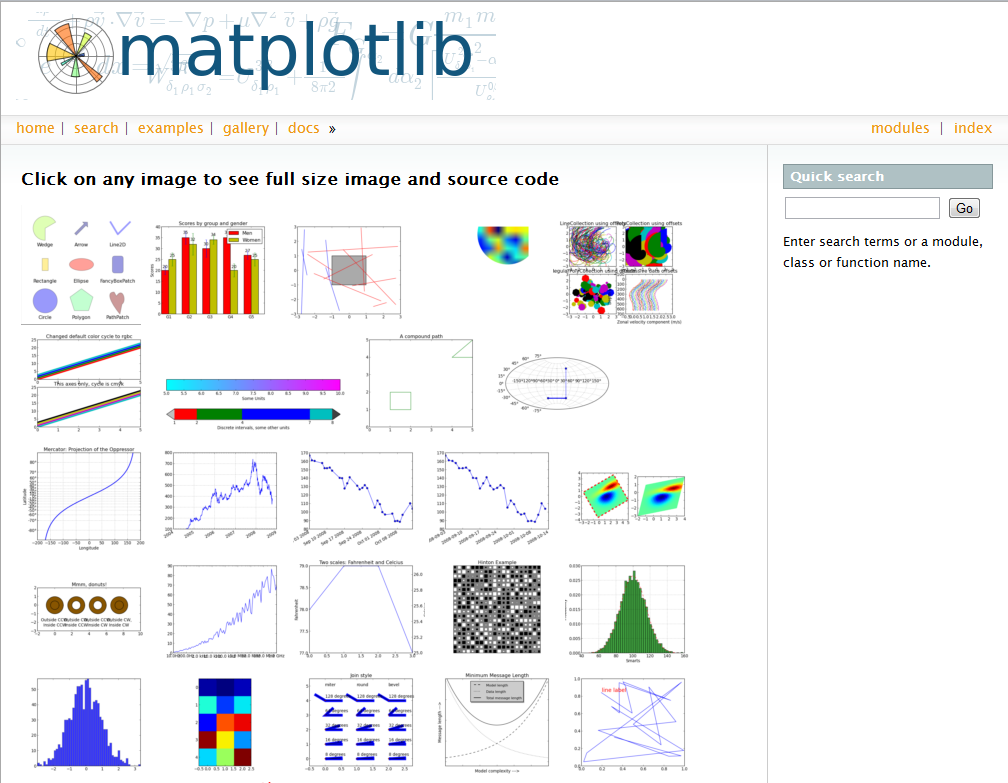
\includegraphics[height=0.6\textheight]{figures/matplotlib_gallery.png}
	\end{figure}
\end{frame}


\section{Creating a simple plot}
\subsection{As simple as it can get}
\begin{frame}{Creating a super simple plot (1)}
  \small{\texttt{SuperSimplePlot.py}}
  \vspace{-15pt}\begin{figure}[ht]
  \centering
        \lstset{numbers=left}
        \lstinputlisting[language=python]{python/SuperSimplePlot.py}
   \end{figure}
\end{frame}

\begin{frame}{Creating a super simple plot (2)}
	\small{\texttt{SuperSimplePlot.py}}
	\vspace{-15pt}\begin{figure}[ht]
		\centering
		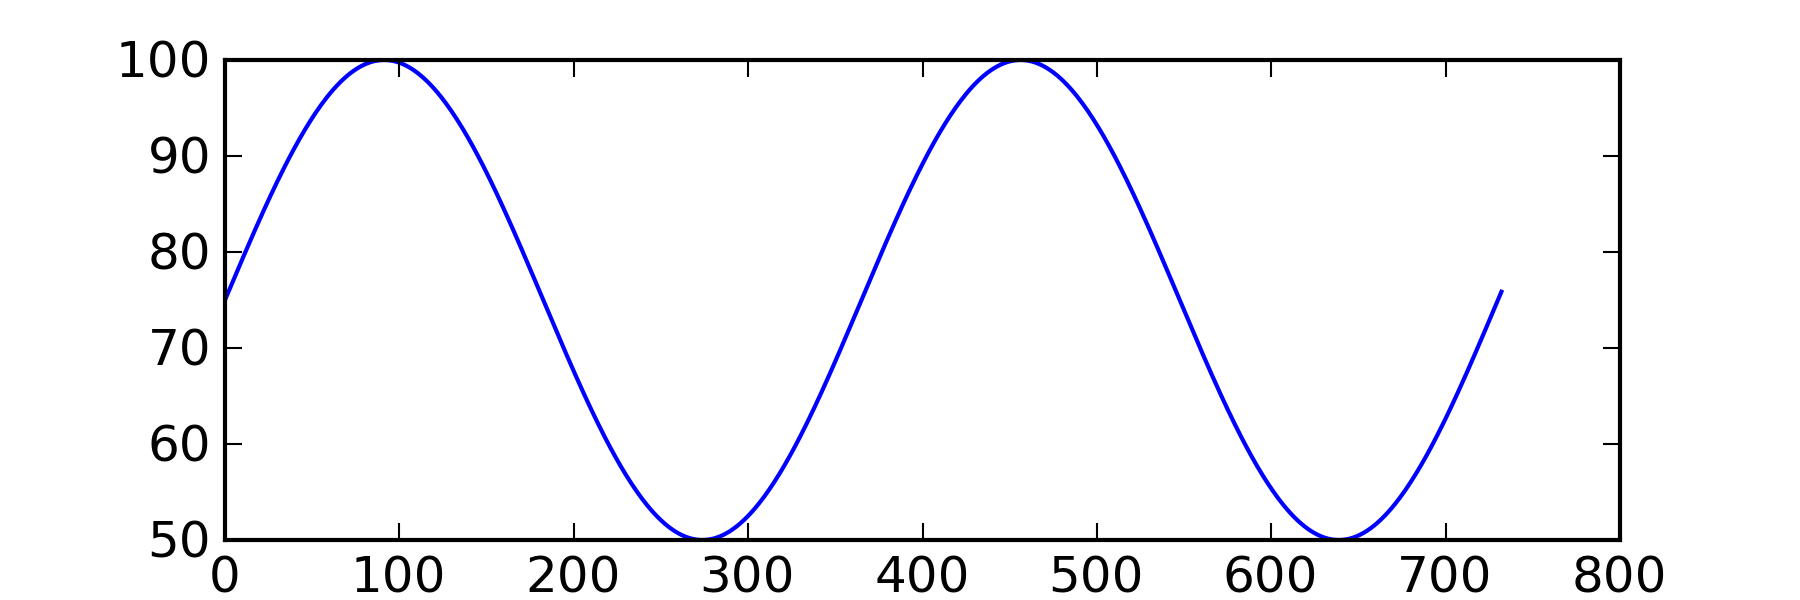
\includegraphics[width=4.5in]{figures/SuperSimplePlot.png}
	\end{figure}
\end{frame}

\begin{frame}{Creating a super simple plot (3)}
	\begin{itemize}
		\item open the command line
		\item type \texttt{python}
		\item enter the text listed below
	\end{itemize}
	\vspace{-15pt}\begin{figure}[ht]
  		\centering
	        \lstinputlisting[language=python]{python/matplotlibInClass.py}
 	\end{figure}
\end{frame}

\begin{frame}{Creating a super simple plot (4)}
	\begin{itemize}
		\item everyone should see...
	\end{itemize}
	\vspace{-15pt}\begin{figure}[ht]
  		\centering
		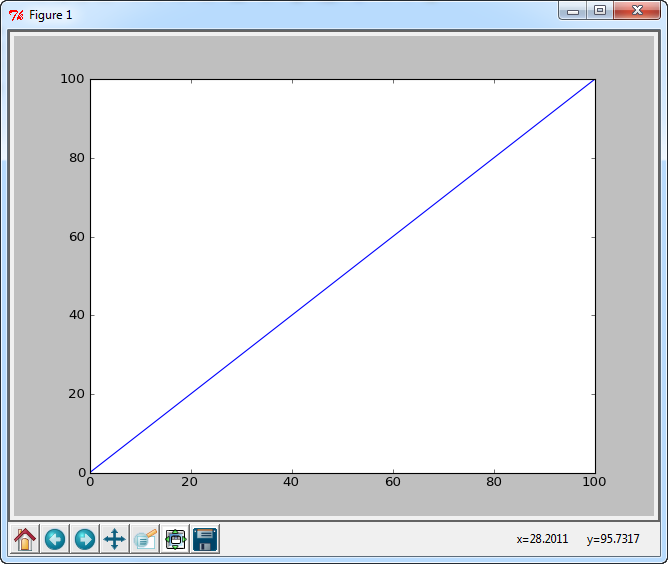
\includegraphics[height=0.70\textheight]{figures/matplotlibInClass.png}
 	\end{figure}
\end{frame}

\subsection{A few preliminaries so we can use the plot in Illustrator}
\begin{frame}{Creating a not so simple plot (1)}
  \small{\texttt{SimplePlot.py}}
  \vspace{-15pt}\begin{figure}[ht]
  \centering
        \lstset{numbers=left}
        \lstinputlisting[language=python, firstline=1,lastline=21,firstnumber=1]{python/SimplePlot.py}
   \end{figure}
\end{frame}

\subsection{Create some data}
\begin{frame}{Creating a not so simple plot (2)}
  \small{\texttt{SimplePlot.py}}
  \vspace{-15pt}\begin{figure}[ht]
  \centering
        \lstset{numbers=left}
        \lstinputlisting[language=python, firstline=22,lastline=36,firstnumber=22]{python/SimplePlot.py}
   \end{figure}
\end{frame}

\subsection{Plot the data with \texttt{matplotlib}}
\begin{frame}{Creating a not so simple plot (3)}
  \small{\texttt{SimplePlot.py}}
  \vspace{-15pt}\begin{figure}[ht]
  \centering
        \lstset{numbers=left}
        \lstinputlisting[language=python, firstline=37,lastline=54,firstnumber=37]{python/SimplePlot.py}
   \end{figure}
\end{frame}

\subsection{Saving the plot}
\begin{frame}{Creating a not so simple plot (4)}
	\small{\texttt{SimplePlot.py}}
	\vspace{-15pt}\begin{figure}[ht]
		\centering
        	\lstset{numbers=left}
        	\lstinputlisting[language=python, firstline=55,lastline=63,firstnumber=55]{python/SimplePlot.py}
	\end{figure}
	\vspace{-30pt}\begin{figure}[ht]
		\centering
		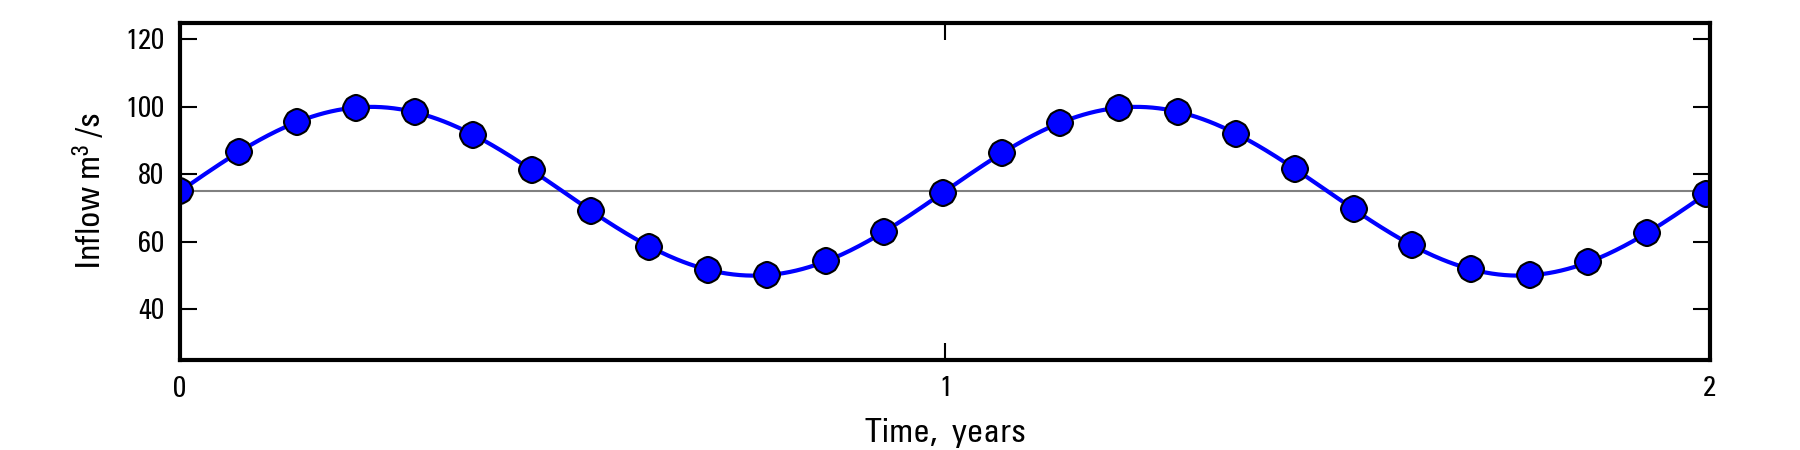
\includegraphics[width=4.5in]{figures/Inflow.png}
	\end{figure}
\end{frame}

\subsection{More plot options}
\begin{frame}{Creating a not so simple plot (5)}
	 \href{http://matplotlib.sourceforge.net/api/pyplot\_api.html\#matplotlib.pyplot.plot}{\texttt{\tiny{\textcolor{blue}{http://matplotlib.sourceforge.net/api/pyplot\_api.html\#matplotlib.pyplot.plot}}}}
	\begin{figure}[ht]
		\centering
		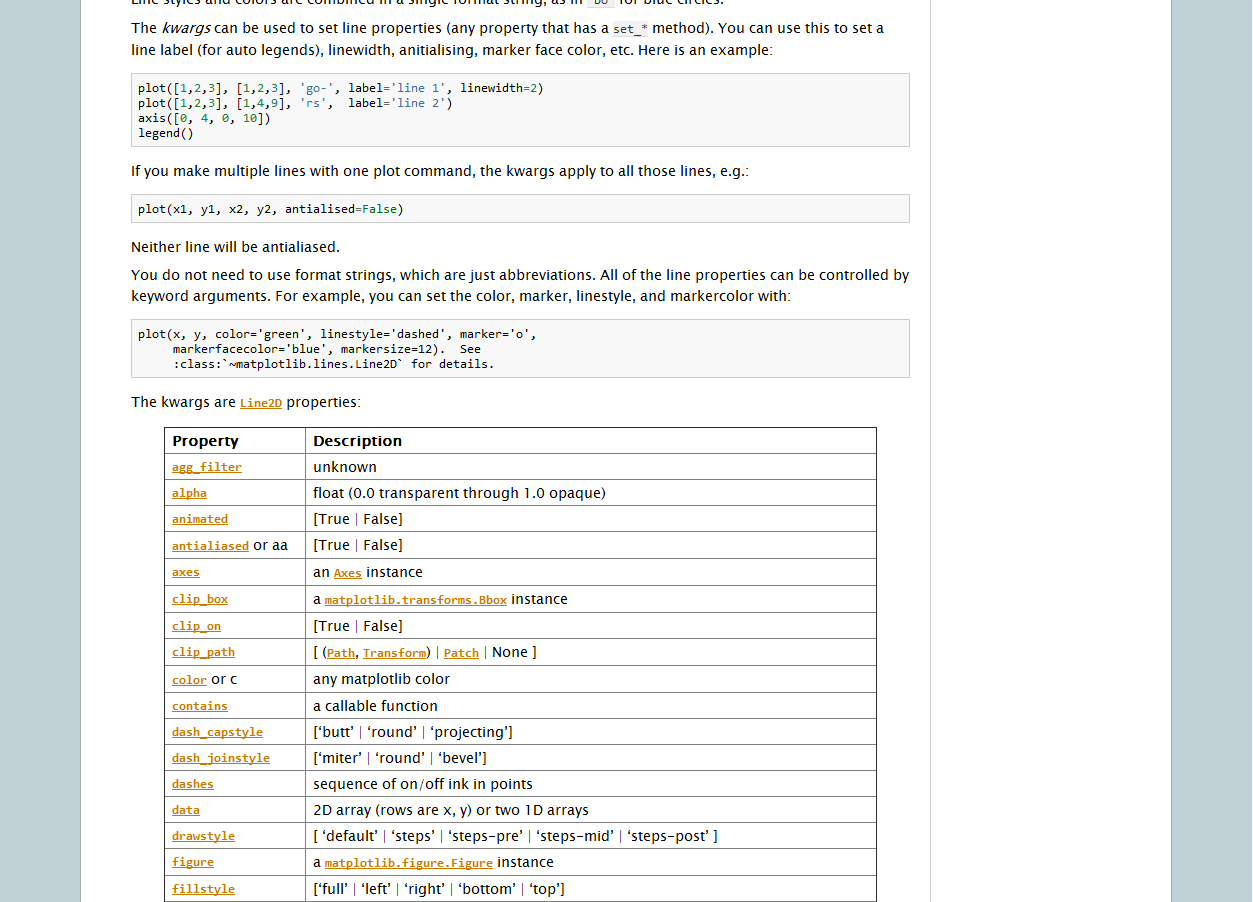
\includegraphics[scale=0.75]{figures/matplotlib_plot_kwargs.png}
	\end{figure}
\end{frame}

\section{Creating a bar chart}
\subsection{Reading \texttt{datetime} data with python}
\begin{frame}{Creating a bar chart (1)}
  \small{\texttt{MeterologicData.csv}}
  \vspace{-15pt}\begin{figure}[ht]
  \centering
        \lstset{numbers=left}
        \lstinputlisting[ firstline=1,lastline=3,firstnumber=1]{data/MeterologicData.csv}
        \lstinputlisting[ firstline=4016,lastline=4018,firstnumber=4016]{data/MeterologicData.csv}
   \end{figure}
  \vspace{-15pt}\small{\texttt{BarChart.py}}
  \vspace{-15pt}\begin{figure}[ht]
  \centering
        \lstset{numbers=left}
        \lstinputlisting[language=python, firstline=26,lastline=33,firstnumber=26]{python/BarChart.py}
        \lstinputlisting[language=python, firstline=9,lastline=11,firstnumber=11]{python/BarChart.py}
   \end{figure}
\end{frame}

\subsection{Working with \texttt{datetime} data}
\begin{frame}{Creating a bar chart (2)}
  \small{\texttt{BarChart.py}}
  \vspace{-15pt}\begin{figure}[ht]
  \centering
        \lstset{numbers=left}
        \lstinputlisting[ firstline=34,lastline=49,firstnumber=49]{python/BarChart.py}
   \end{figure}
\end{frame}

\subsection{\texttt{matplotlib} subplots}
\begin{frame}{Creating a bar chart (3)}
  \small{\texttt{BarChart.py}}
  \vspace{-15pt}\begin{figure}[ht]
  \centering
        \lstset{numbers=left}
        \lstinputlisting[ firstline=57,lastline=78,firstnumber=57]{python/BarChart.py}
   \end{figure}
\end{frame}

\subsection{Final bar chart}
	\begin{frame}{Creating a bar chart (4)}
		\vspace{-15pt}\begin{figure}[ht]
		\centering
		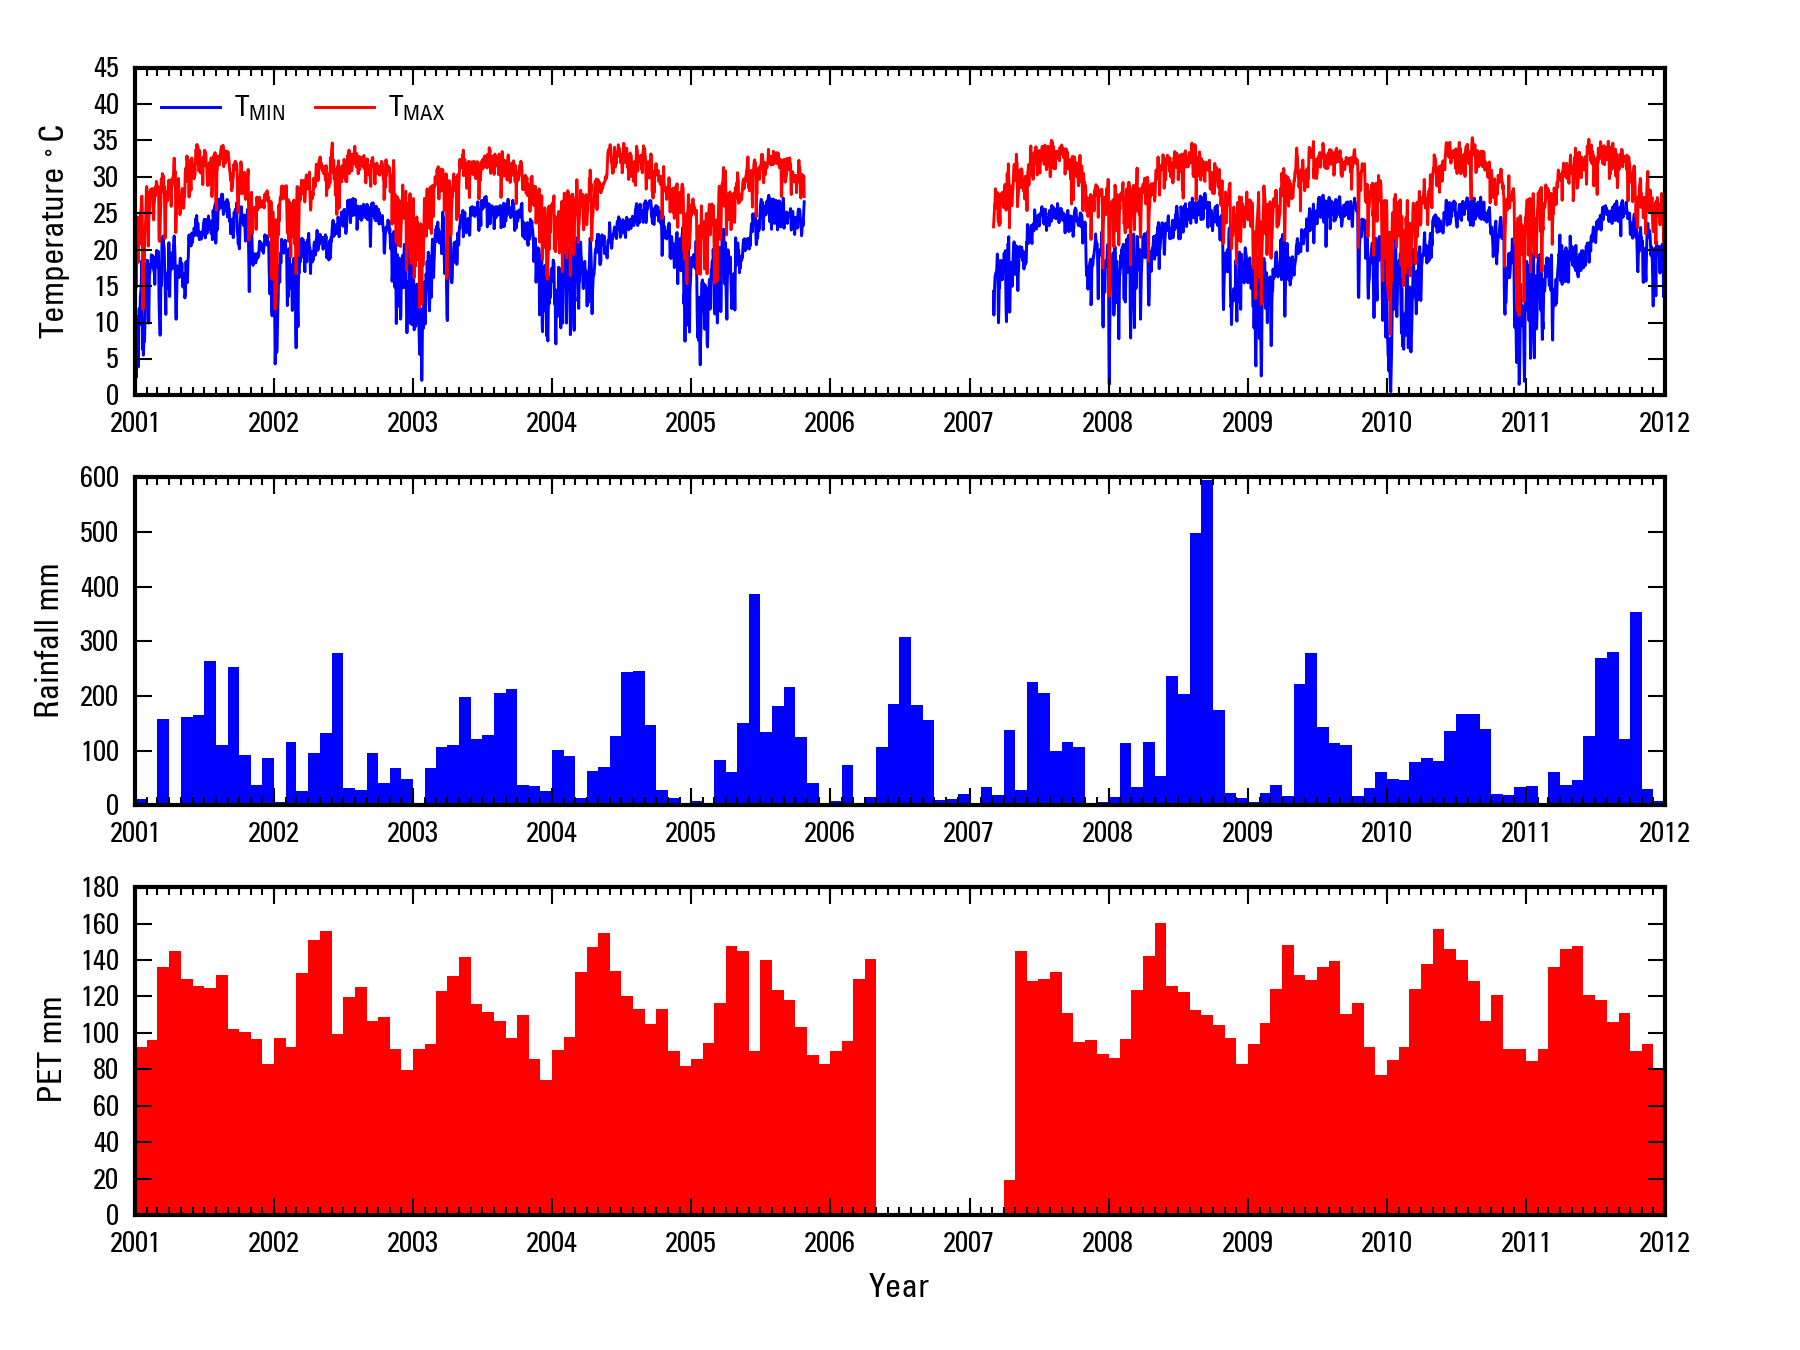
\includegraphics[width=0.75\textwidth]{figures/MeterologicBar.png}
	\end{figure}
\end{frame}

\section{Maps from model results}
\subsection{Define dimensions of model}
	\begin{frame}{Model coordinates}
		\small{\texttt{plotHeads.py}}
		\vspace{-15pt}\begin{figure}[ht]
		\centering
		\lstset{numbers=left}
		\lstinputlisting[language=python, firstline=27,lastline=42,firstnumber=27]{python/plotHeads.py}
	\end{figure}
\end{frame}

\subsection{Reading binary head file}
\begin{frame}{Binary head data}
	\small{\texttt{plotHeads.py}}
	\vspace{-15pt}\begin{figure}[ht]
		\centering
		\lstset{numbers=left}
		\lstinputlisting[language=python, firstline=43,lastline=49,firstnumber=43]{python/plotHeads.py}
		\lstinputlisting[language=python, firstline=55,lastline=63,firstnumber=55]{python/plotHeads.py}	
	\end{figure}
\end{frame}

\subsection{Plotting a map with contours}
\begin{frame}{Create the map (1)}
	\small{\texttt{plotHeads.py}}
	\vspace{-15pt}\begin{figure}[ht]
		\centering
	        \lstset{numbers=left}
	       	\lstinputlisting[language=python, firstline=64,lastline=66,firstnumber=64]{python/plotHeads.py}
	       	\lstinputlisting[language=python, firstline=72,lastline=83,firstnumber=72]{python/plotHeads.py}
	\end{figure}
\end{frame}

\begin{frame}{Create the map (2)}
	\small{\texttt{plotHeads.py}}
	\vspace{-15pt}\begin{figure}[ht]
		\centering
	        \lstset{numbers=left}
	       	\lstinputlisting[language=python, firstline=84,lastline=100,firstnumber=84]{python/plotHeads.py}
	\end{figure}
\end{frame}

\begin{frame}{Final maps}
	\begin{figure}[ht]
		\centering
	       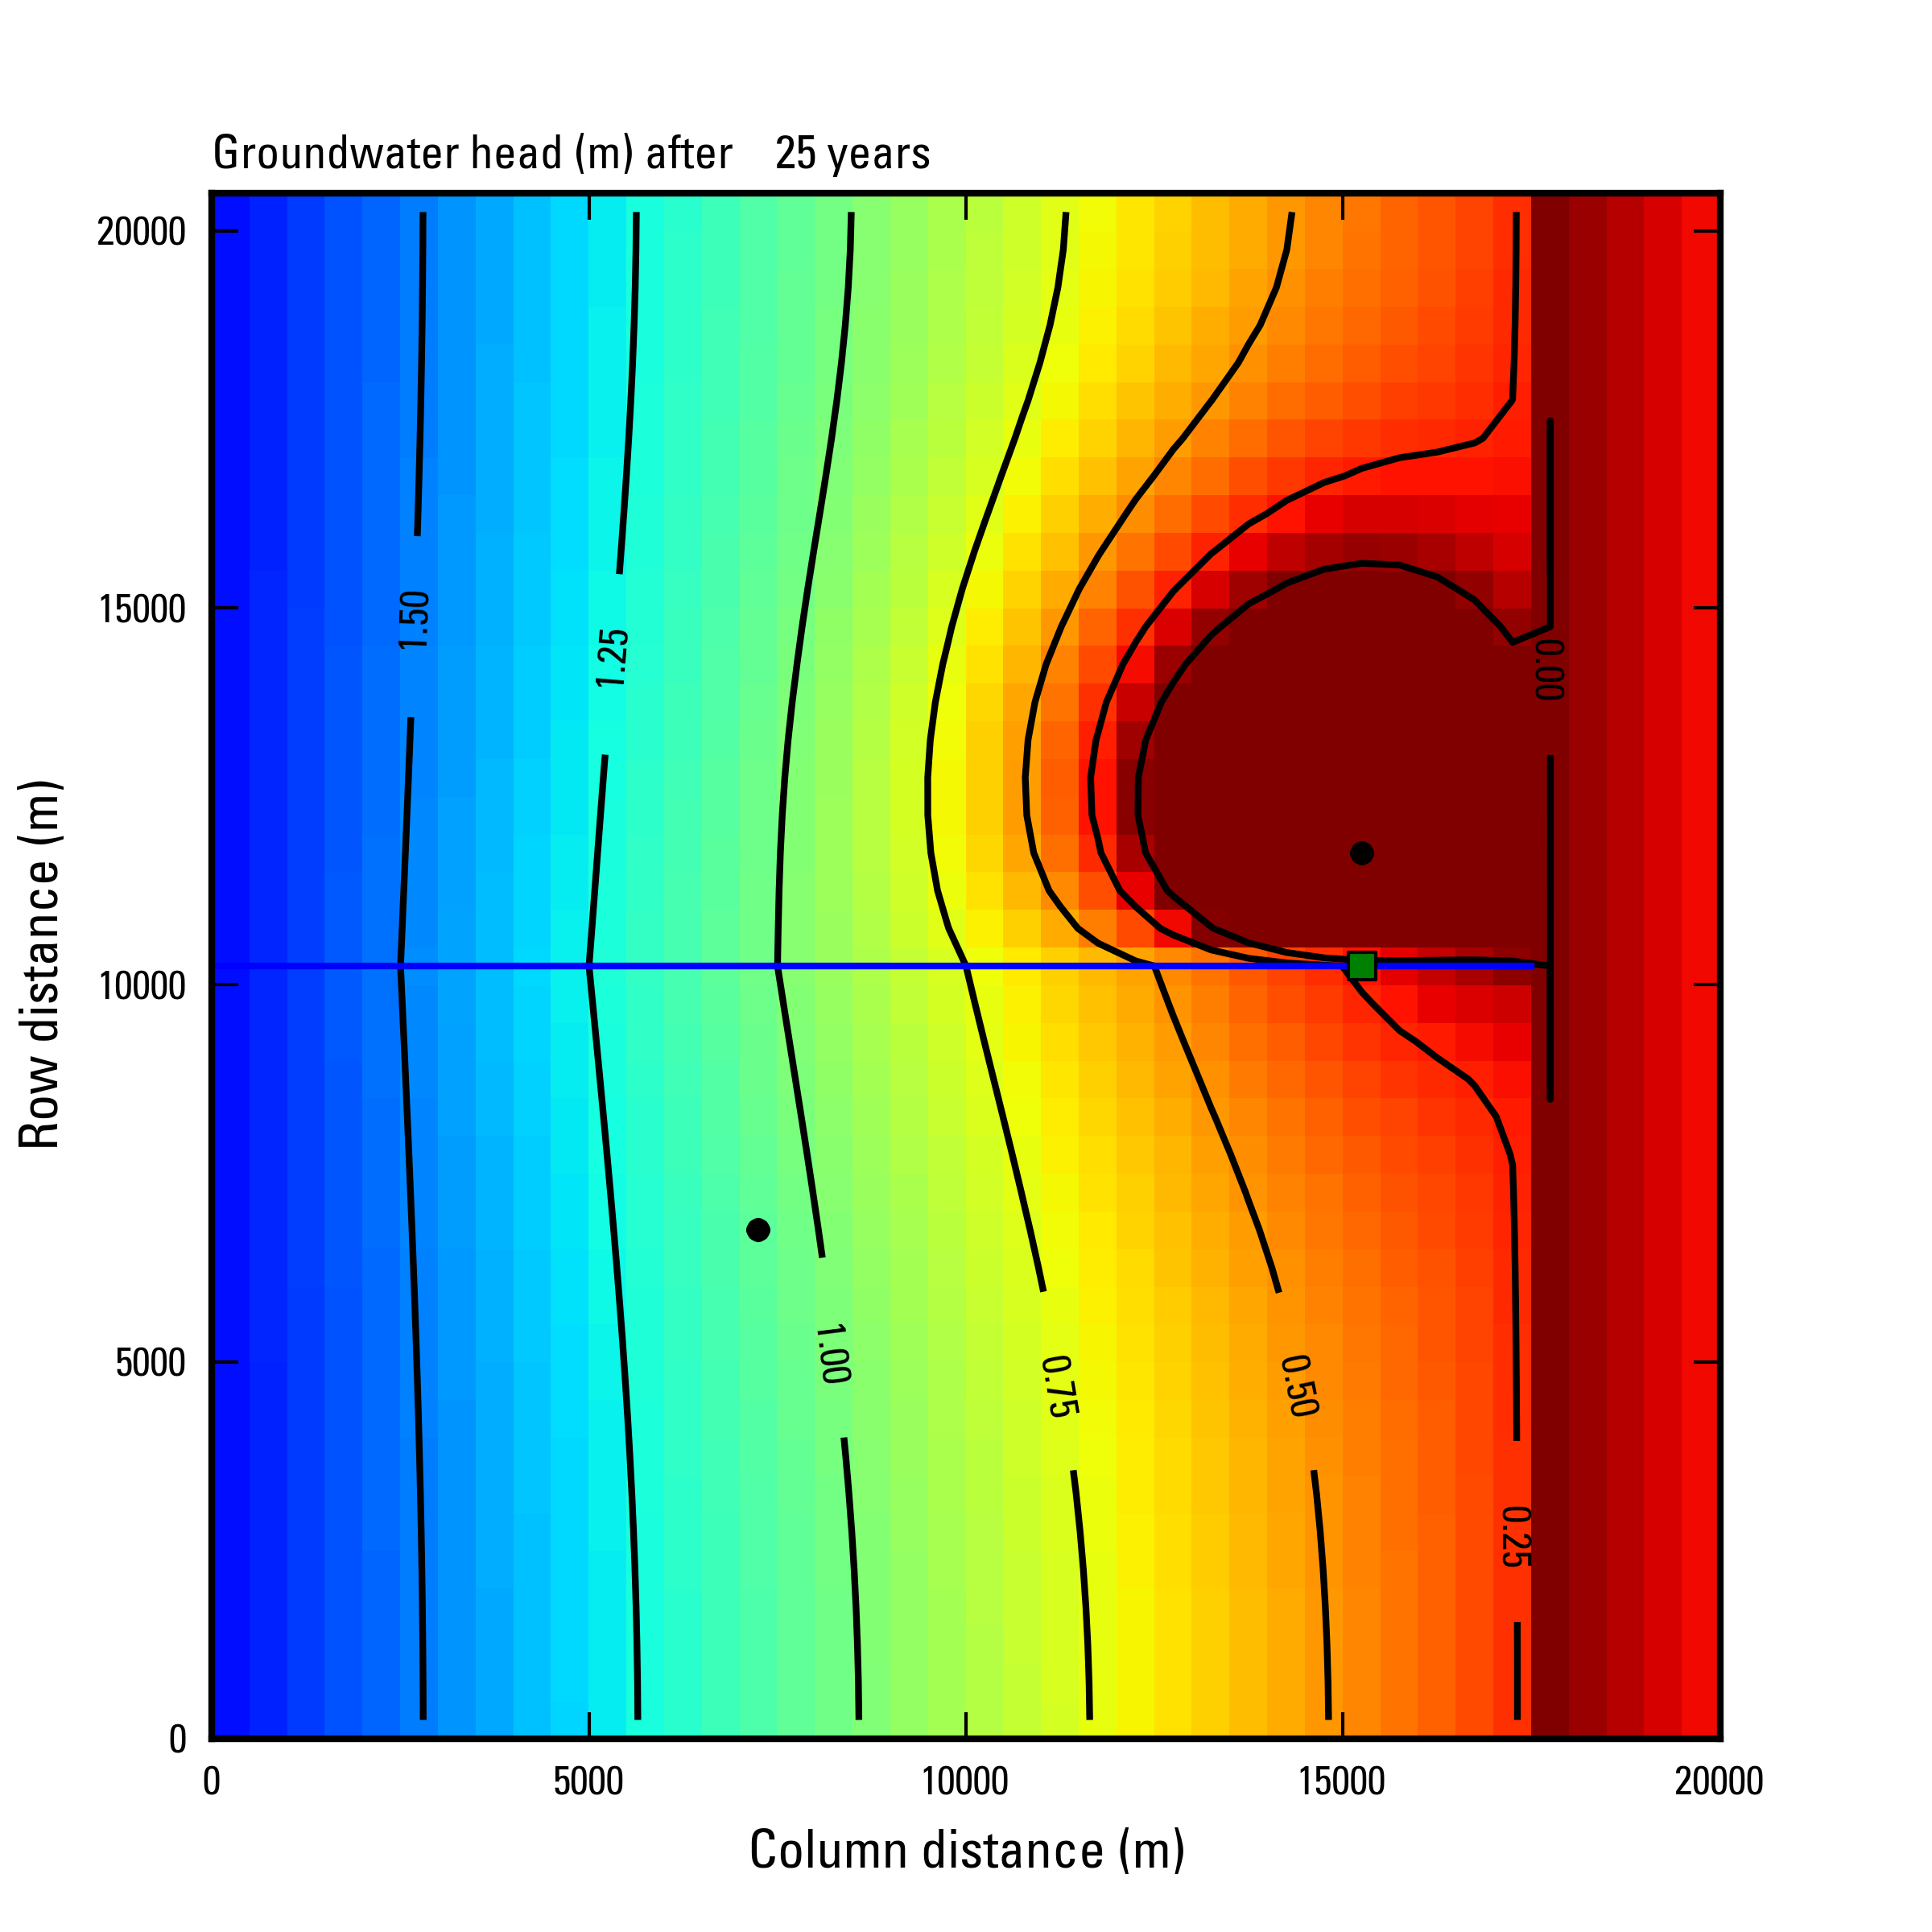
\includegraphics[width=0.5\textwidth]{figures/MF_Results_00024.png} 
	       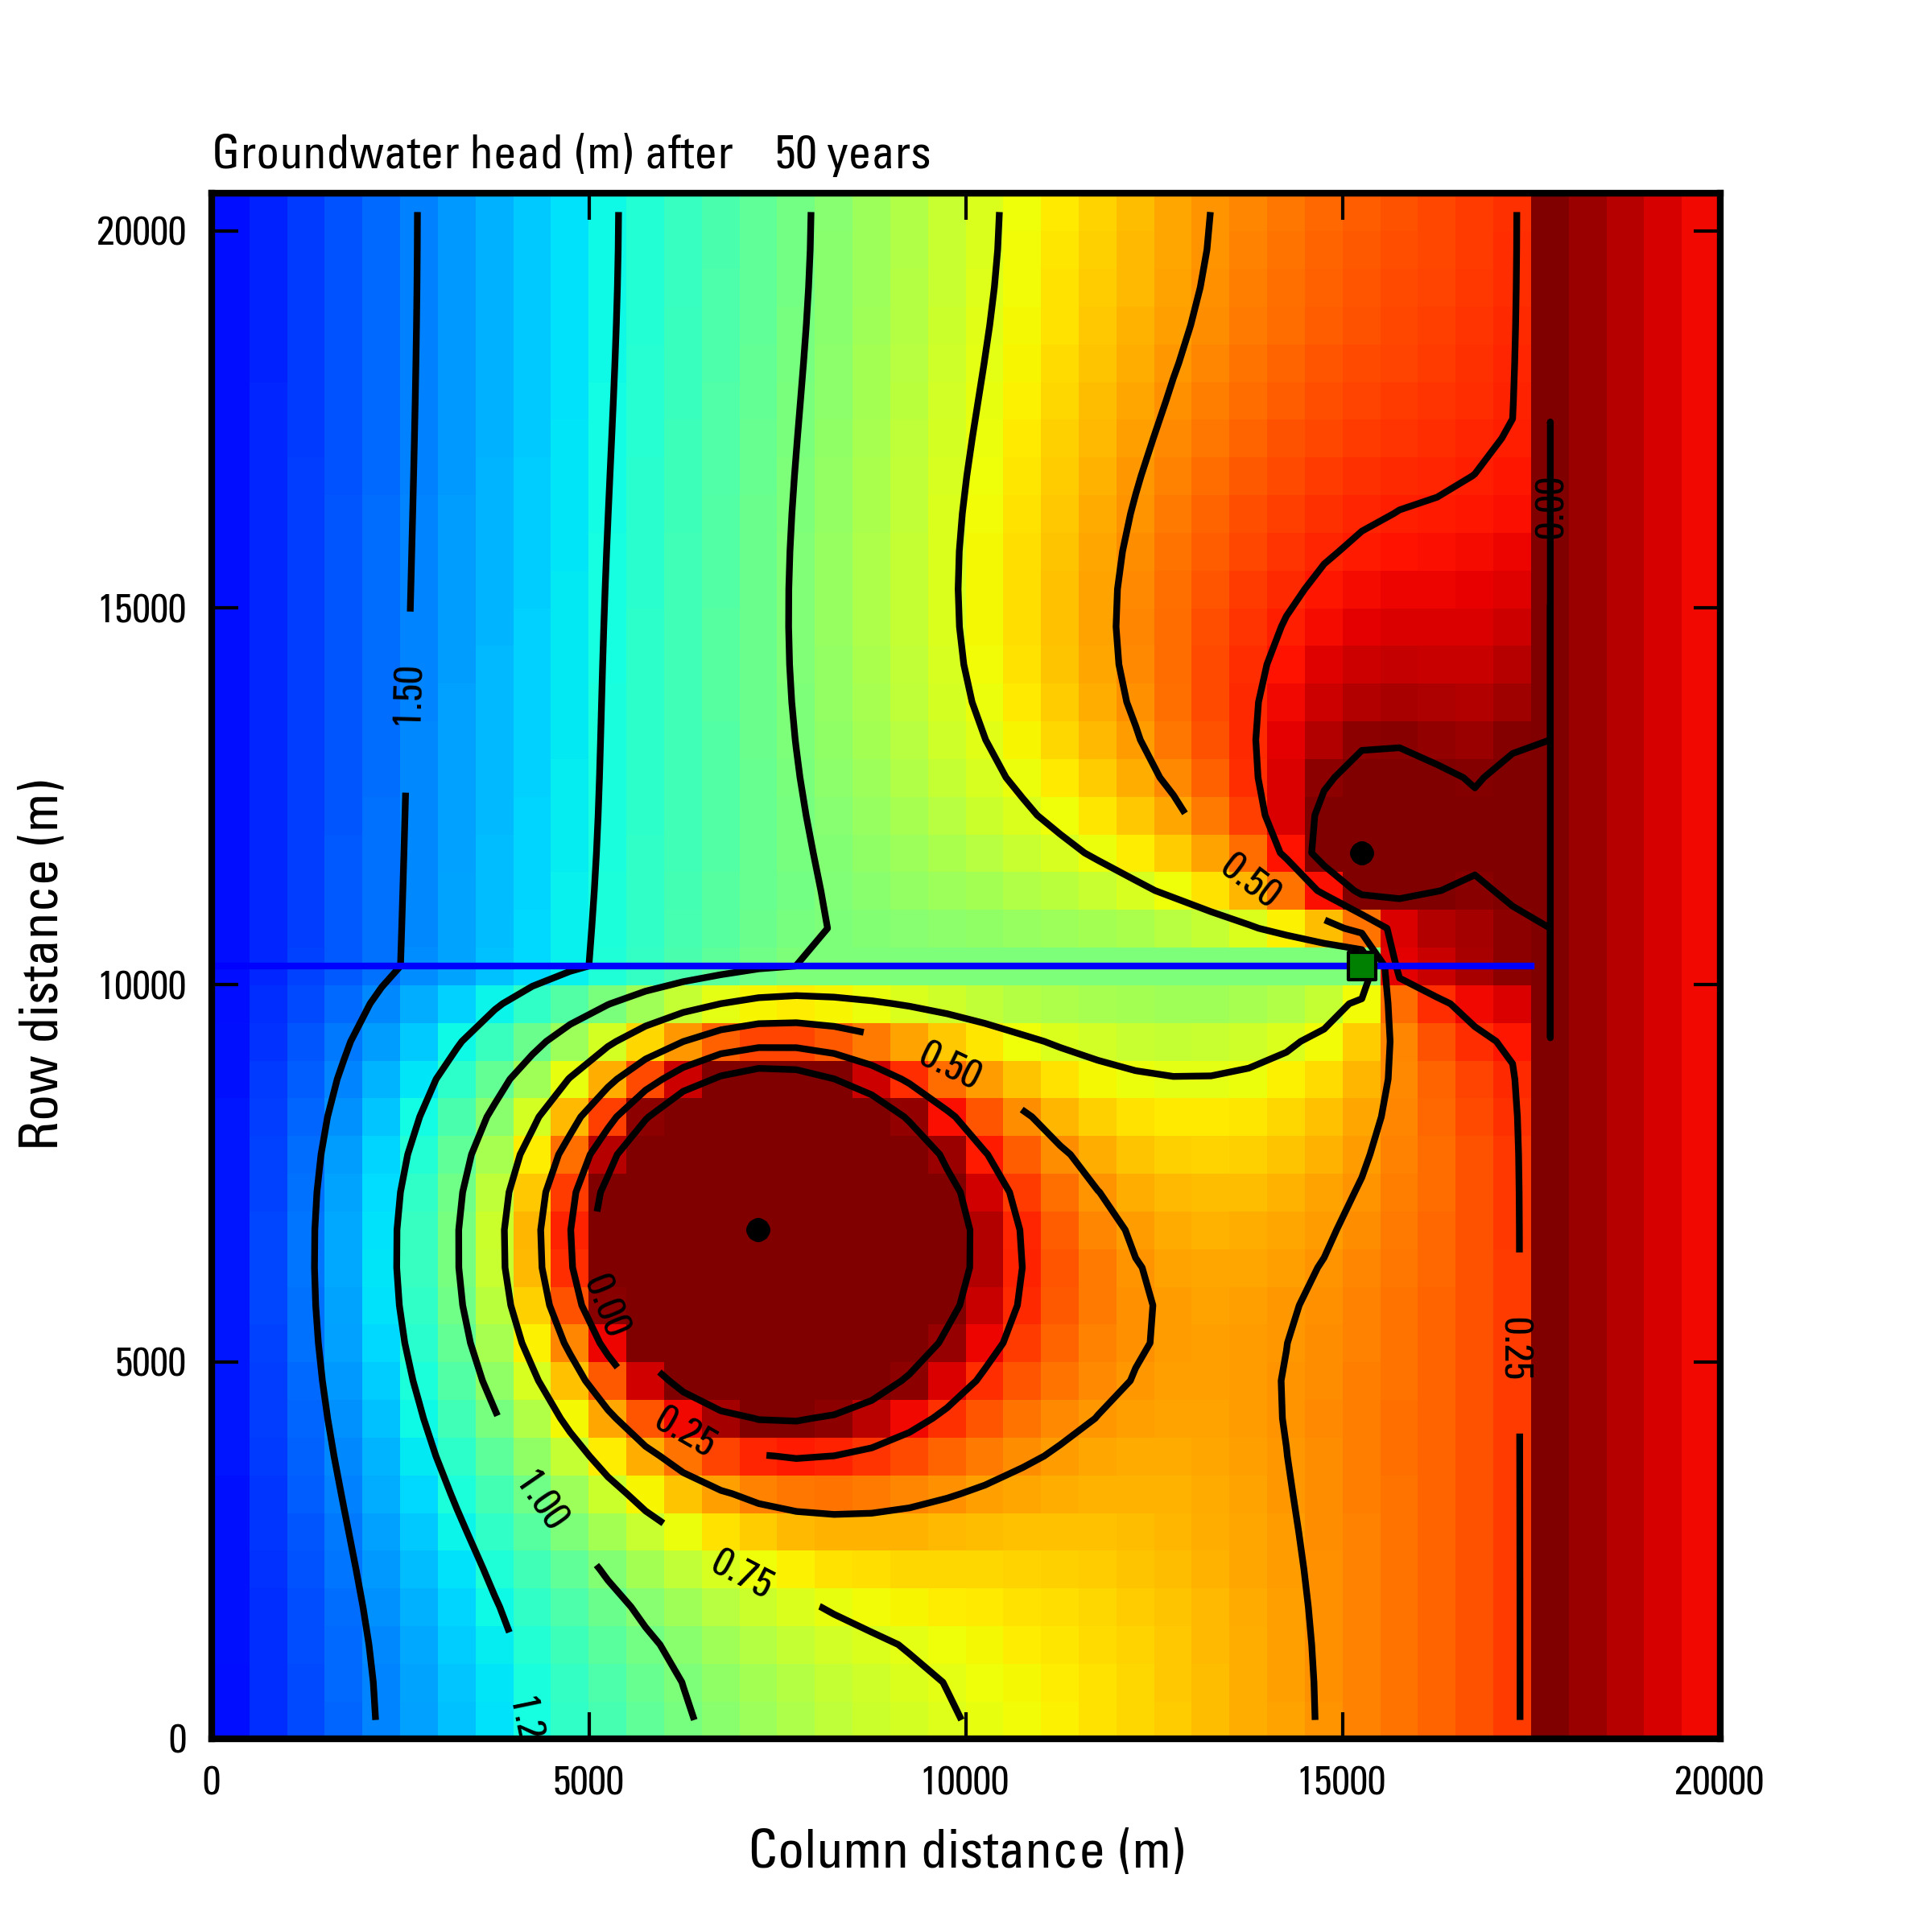
\includegraphics[width=0.5\textwidth]{figures/MF_Results_00049.png}
	 \end{figure}
\end{frame}

\section{Animations}
\subsection{How to make an animation}
\begin{frame}{Using \texttt{ffmpeg.exe}}
\small{\texttt{plotHeads.py}}
	\vspace{-15pt}\begin{figure}[ht]
		\centering
	        \lstset{numbers=left}
	        \lstinputlisting[language=python, firstline=1,lastline=3,firstnumber=1]{python/plotHeads.py}
	        \lstinputlisting[language=python, firstline=101,lastline=111,firstnumber=101]{python/plotHeads.py}
	\end{figure}
\end{frame}

\subsection{Final animation}
\begin{frame}{Using \texttt{ffmpeg.exe}}
	\begin{center}
	\includemedia[
activate=onclick,width=0.8\textheight]{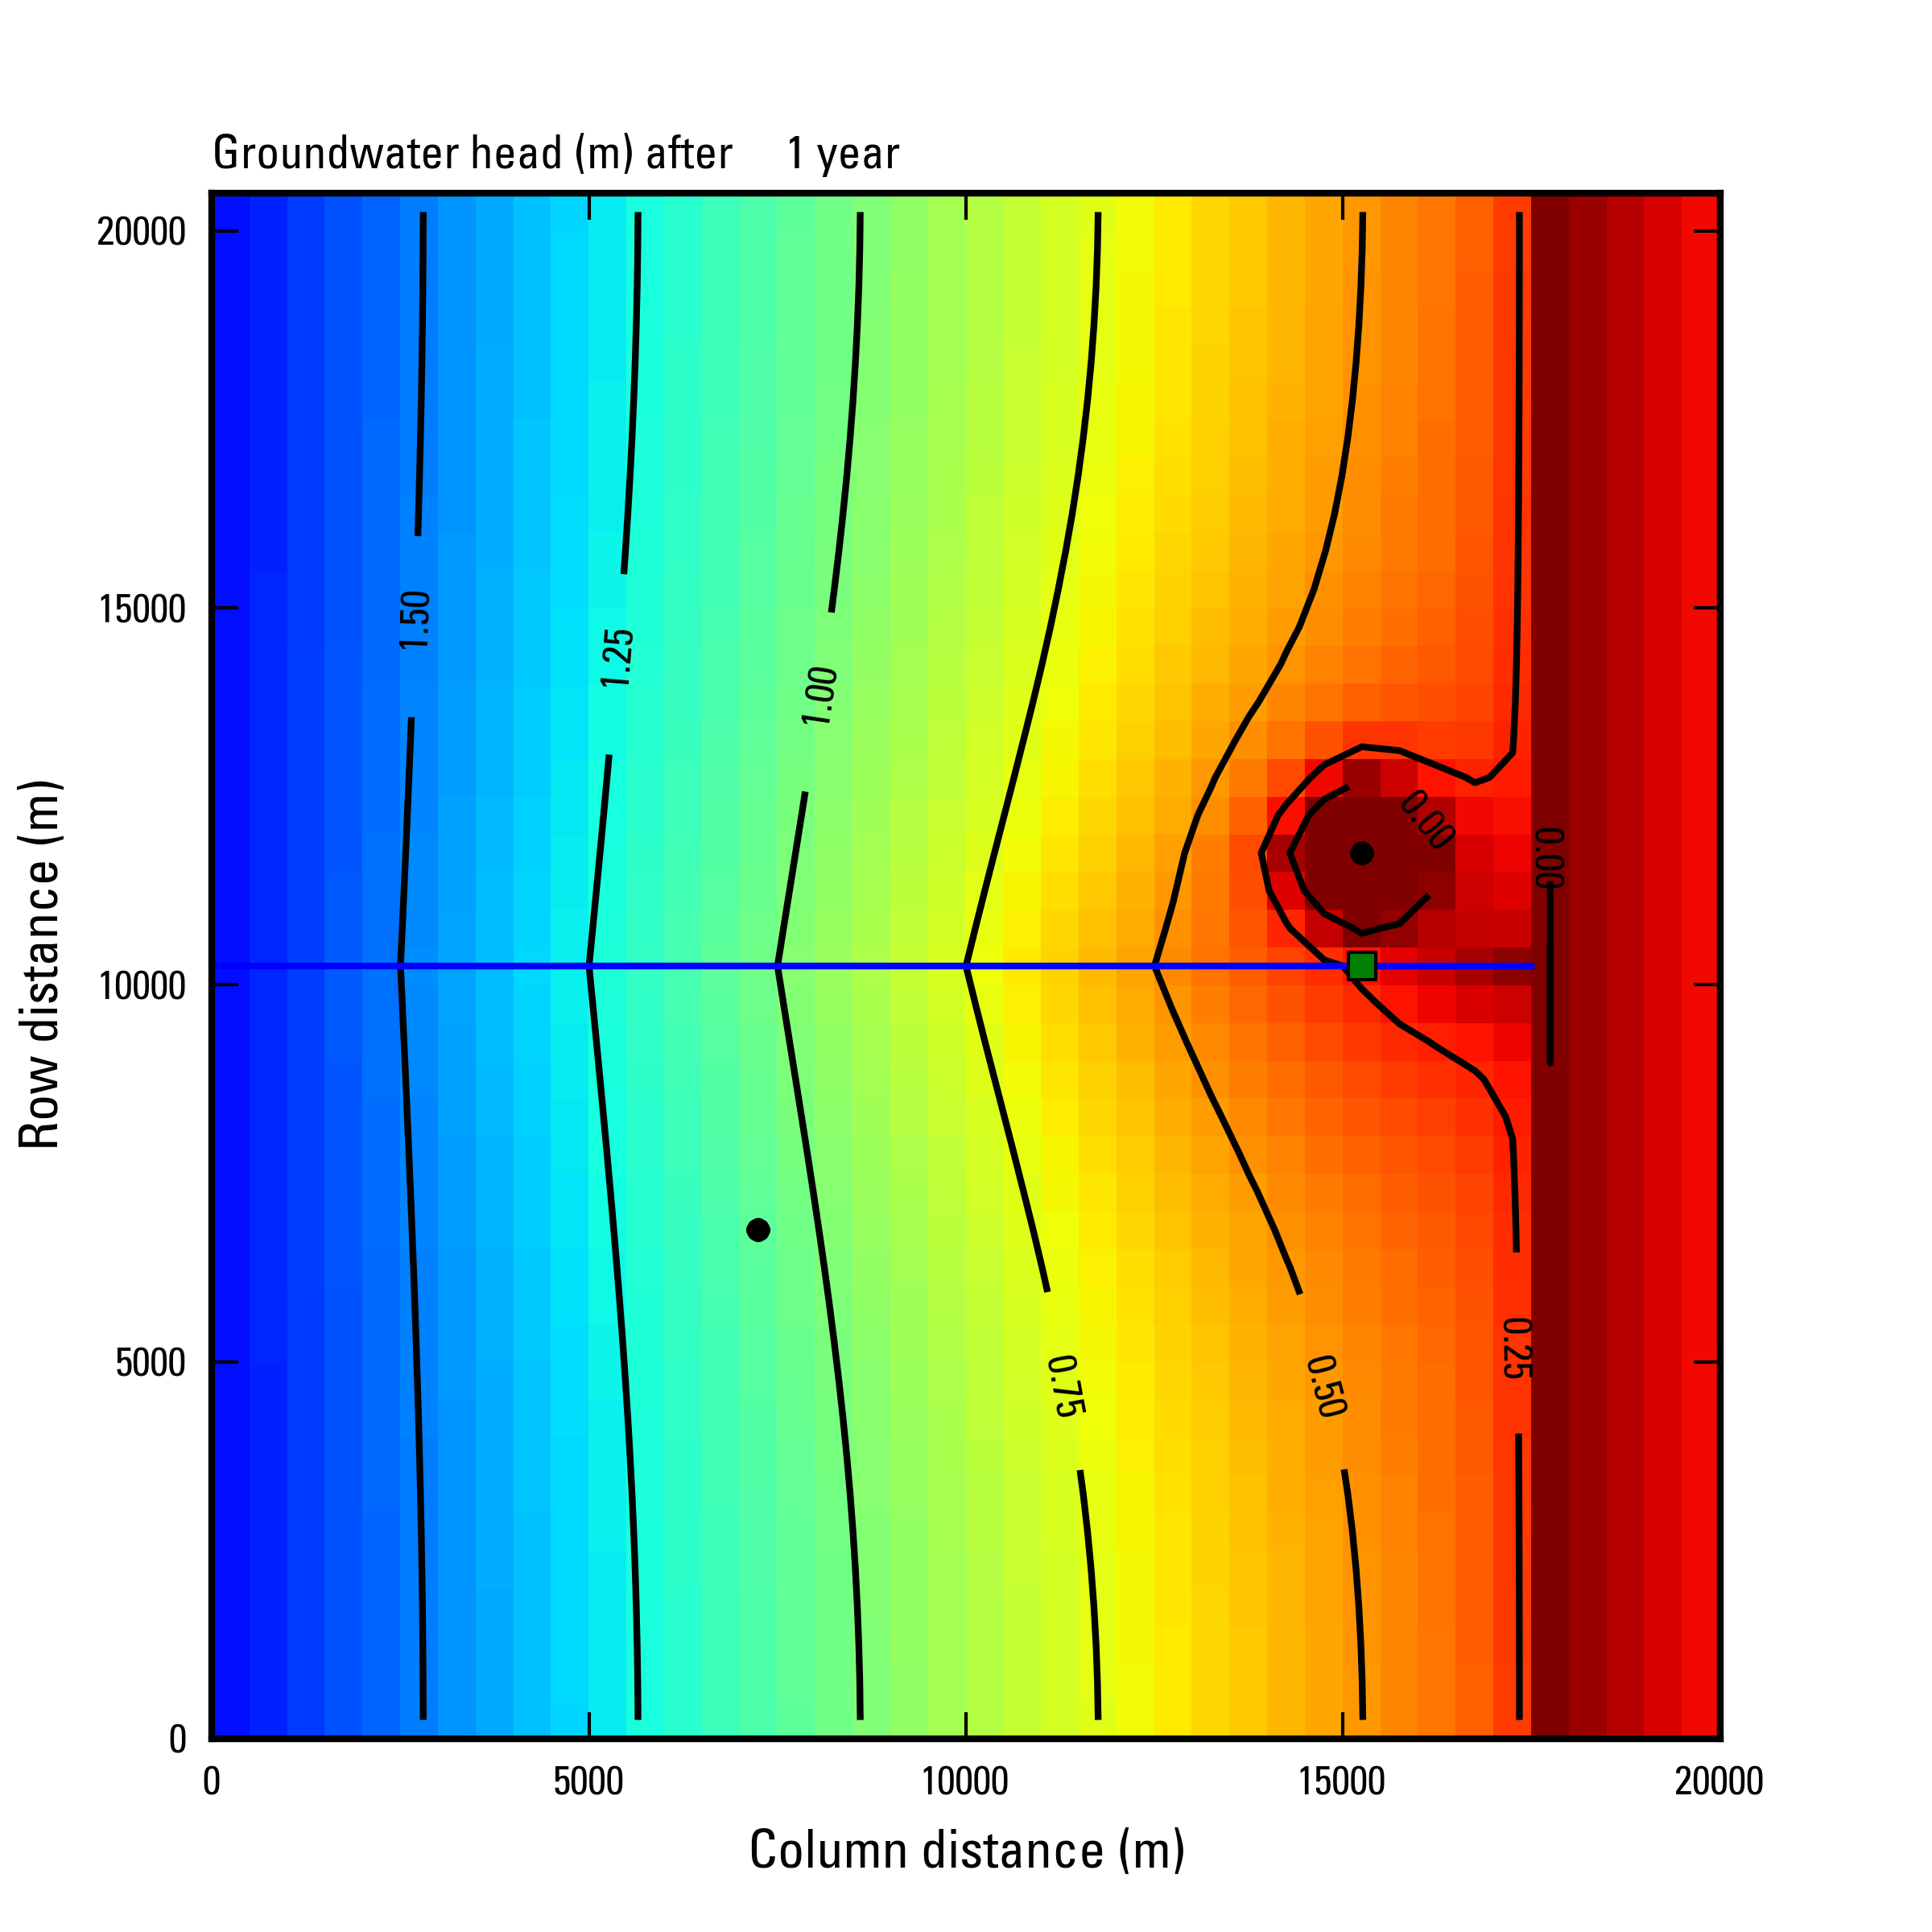
\includegraphics[height=0.8\textheight]{figures/MF_Results_00000.png}}{figures/MF_Results.swf}
	\end{center}
\end{frame}

\section{Extras}
\subsection{Cross-sections}
\begin{frame}{Adding cross-sections (1)}
	\small{\texttt{Cross-sectionSample.py}}
	\vspace{-15pt}\begin{figure}[ht]
		\centering
	        \lstset{numbers=left}
	        \lstinputlisting[language=python]{python/Cross-sectionSample.py}
	\end{figure}
\end{frame}

\begin{frame}{Adding cross-sections (2)}
	\vspace{-10pt}\begin{figure}[ht]
		\centering
		\hspace{20pt}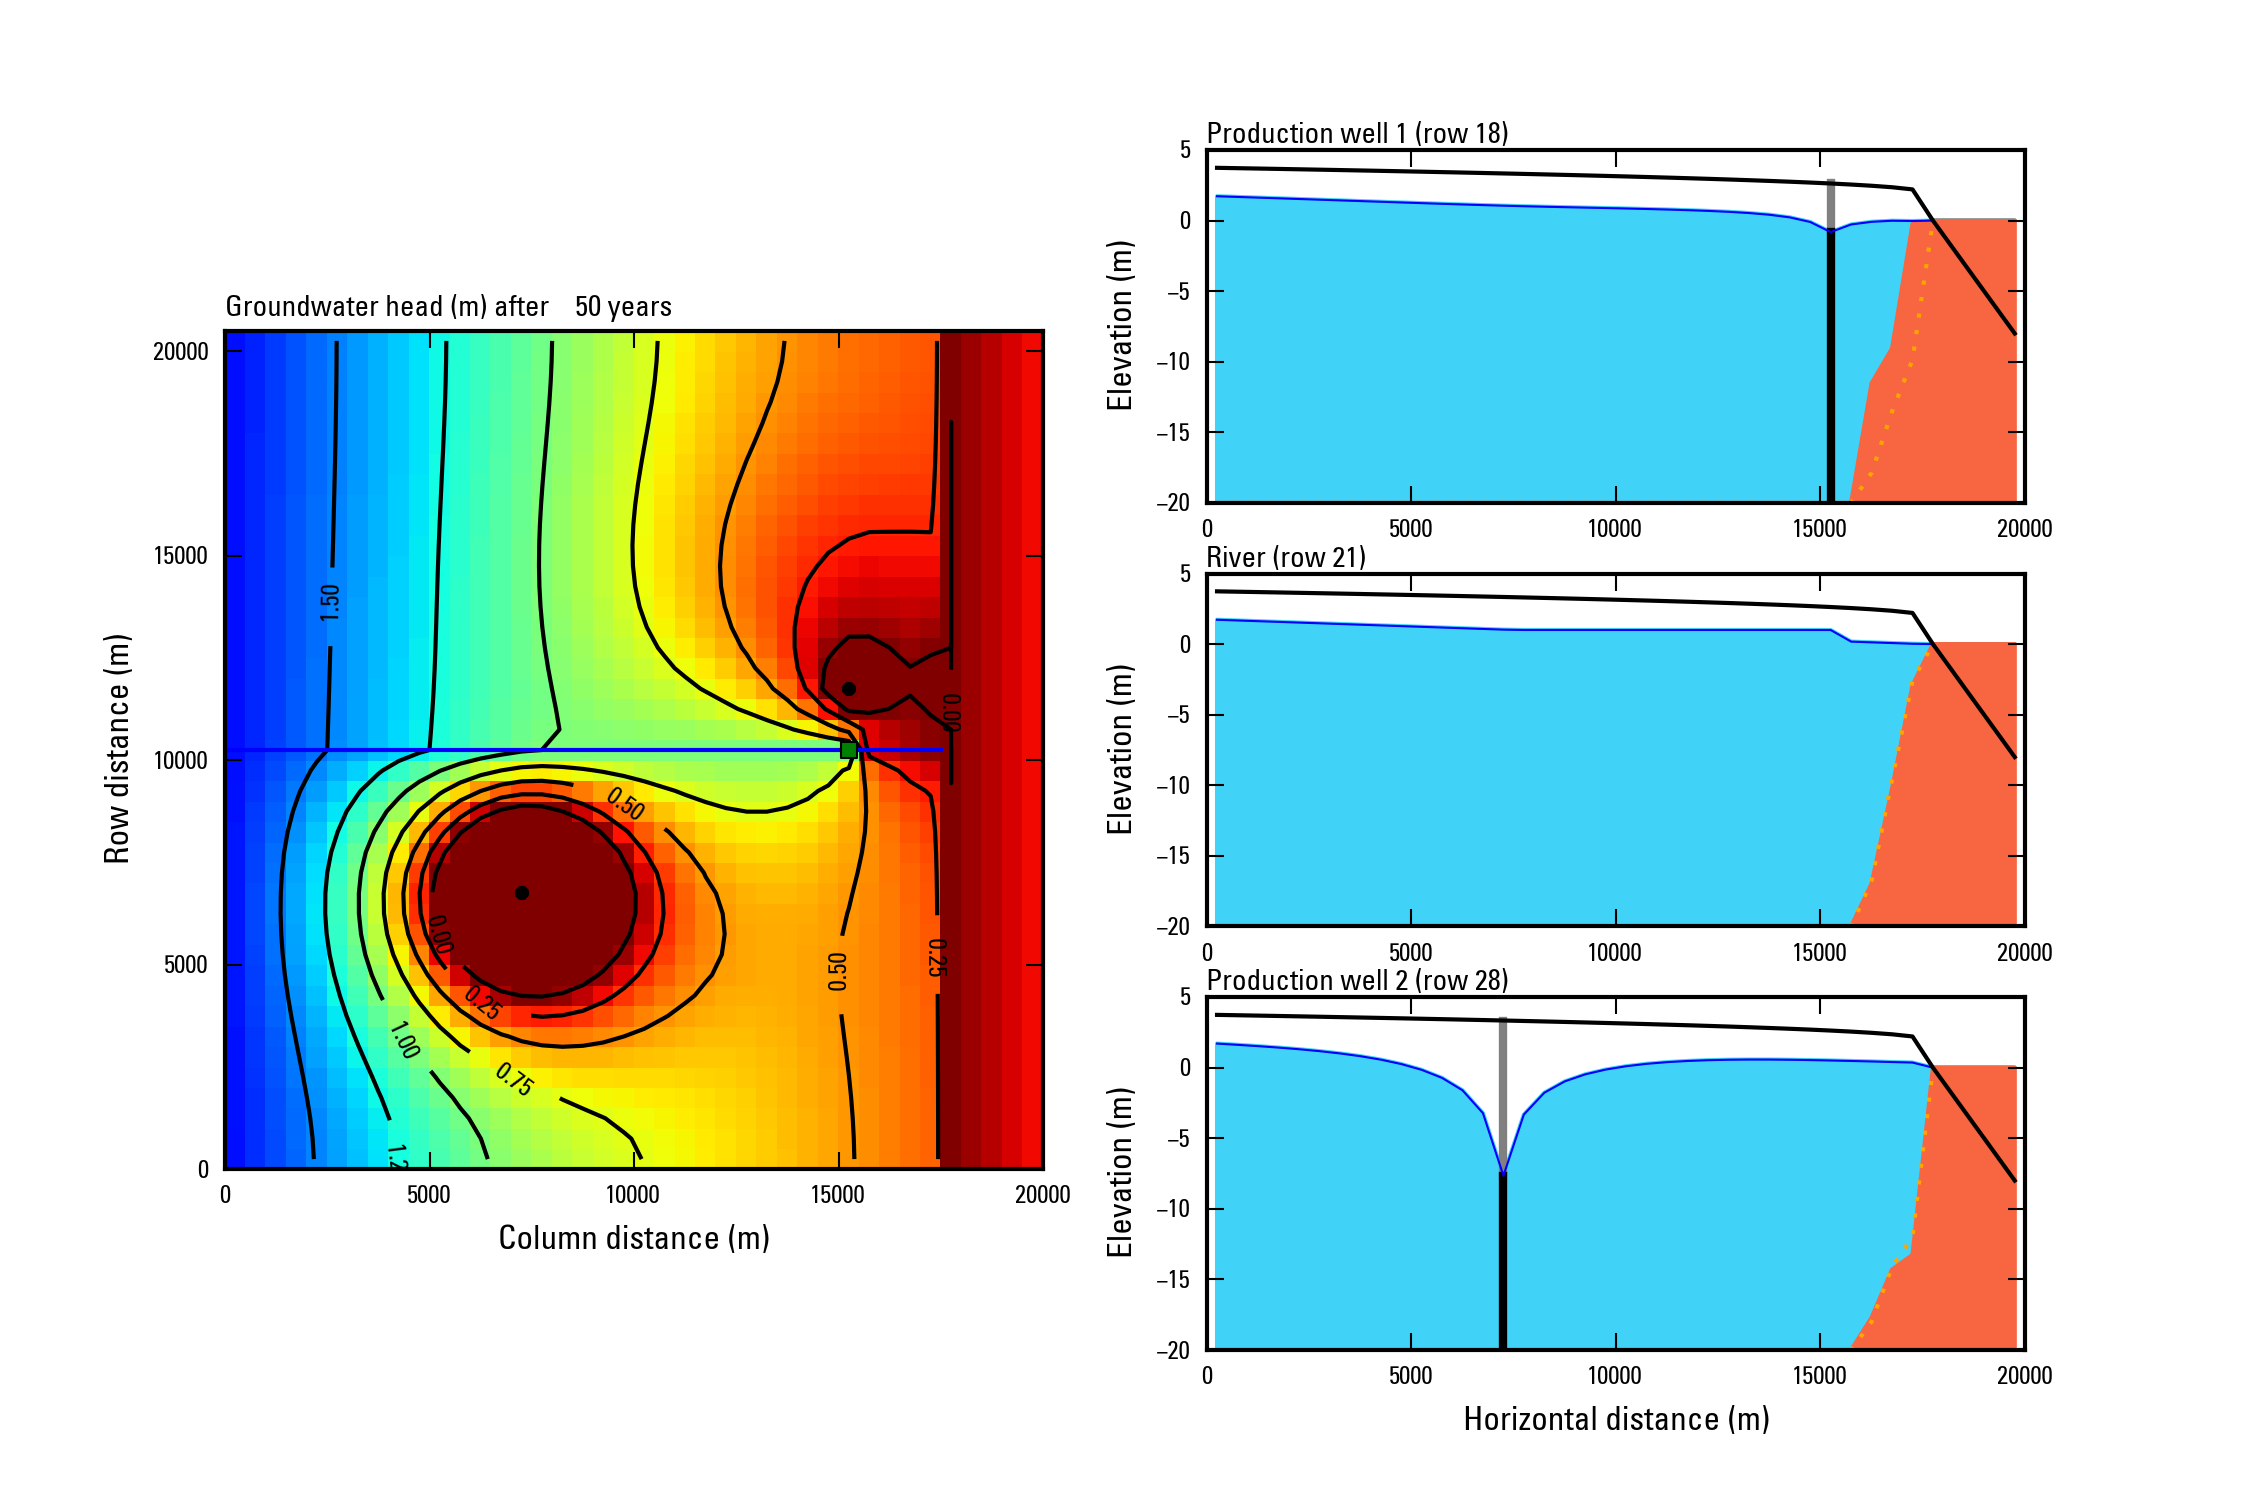
\includegraphics[width=0.90\textwidth]{figures/SWI_Results_0000054750.png} 
	 \end{figure}
\end{frame}

\subsection{Automation}
\begin{frame}{Automating model runs and figure preparation}
	\small{\texttt{AutomationSample.bat}}
	\vspace{-15pt}\begin{figure}[ht]
		\centering
	        \lstset{numbers=left}
	        \lstinputlisting[language=python, firstline=1,lastline=21,firstnumber=1]{data/AutomationSample.bat}
	\end{figure}
\end{frame}


\end{document}